\documentclass{beamer}

\usepackage{graphicx}
\usepackage{mathtools}
\usepackage{xifthen}
\usepackage{tikz}
\usetikzlibrary{positioning}
\usetikzlibrary {graphs.standard}

\tikzstyle{vertex}=[draw, circle, fill=black, inner sep=0.4mm]


\newcommand{\declarefunction}[2][]{%
    \ifthenelse{\isempty{#1}}{%
        \expandafter\newcommand\csname #2\endcsname{\mathsf{#2}}%
    }{%
        \expandafter\newcommand\csname #1\endcsname{\mathsf{#2}}%
    }%
}

\declarefunction{thin}
\declarefunction{cm}
\declarefunction{tw}
\declarefunction{pw}
\declarefunction{mw}
\declarefunction{s}
\declarefunction{nd}
\declarefunction{tc}
\declarefunction{vs}
\declarefunction{vc}
\declarefunction{p}

\DeclarePairedDelimiter\abs{\lvert}{\rvert}

\newcommand{\vimage}[2][]{\vcenter{\hbox{\includegraphics[#1]{#2}}}}
\newcommand{\varrow}{\vcenter{\hbox{\scalebox{2}{$\rightarrow$}}}}

\usetheme{Warsaw}

\title[Param. algorithms for \text{Thinness} via the cluster module number]{Parameterized algorithms for \textsc{Thinness} via the cluster module number}
\author{Flavia Bonomo, Eric Brandwein, Ignasi Sau}
\institute{Group: Graph Theory and Combinatorial Optimization}
\date{March 11th, 2024}

\begin{document}

\AtBeginSection[]
{{
    \definecolor{ceruleanblue}{rgb}{0.23, 0.28, 0.75}
    \setbeamertemplate{background canvas}{%
    \begin{tikzpicture}[remember picture,overlay]
    \shade[top color=ceruleanblue,bottom color=black,middle color=ceruleanblue]
    (current page.north west)
        rectangle
    (current page.south east);
    \end{tikzpicture}%     
    }
    \setbeamercolor{background canvas}{bg=ceruleanblue}
    \begin{frame}[plain]
        \usebeamerfont{title}
        {\huge
        \textcolor{white}{\insertsectionhead}
        }
        
    \end{frame}
}}

\frame{\titlepage}


\begin{frame}
    \frametitle{Table of Contents}
    \tableofcontents[hideallsubsections]
\end{frame}

\section{Thinness}
\subsection{Definition}
\begin{frame}{Consistent solution}
    A \emph{consistent solution using $k$ classes} for a graph $G$ is a pair $(\prec, S)$ where 
    \begin{itemize}
        \item $\prec$ is a strict total order on $V(G)$, and 
        \item $S$ is a partition of $V(G)$ into $k$ classes,
    \end{itemize}
    such that, for each triple of vertices $u\prec v \prec w$ of $G$, if
    \begin{itemize}
        \item $u$ and $v$ belong to the same class in $S$, and
        \item $(u,w) \in E(G)$,
    \end{itemize}
    then $(v,w) \in E(G)$.
\end{frame}

\begin{frame}{Thinness}
    \begin{center}
        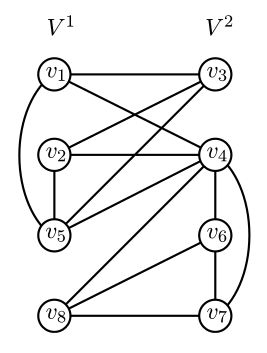
\includegraphics[width=0.4\textwidth]{img/ejemplo_thinness.png}
    \end{center}
\end{frame}

\begin{frame}{Definition}
    A graph is \emph{$k$-thin} if it admits a consistent solution using $k$ classes.
    The \emph{thinness} of a graph $G$, denoted by $\thin(G)$, is the minimum integer $k$ such that $G$ admits a consistent solution using $k$ classes.
    \vspace{1em}
    \begin{block}{\textsc{Thinness} problem}
        \textbf{Input:} A graph $G$ and an integer $k$.

        \textbf{Output:} Is $\thin(G) \leq k$?
    \end{block}
\end{frame}


\subsection{Complexity}
\begin{frame}{Thinness}
    \begin{block}{Theorem (Y. Shitov, \cite{thinness-np-complete})}
        \textsc{Thinness} is NP-complete.
    \end{block}
    \pause
    \vspace{1em}
    \textbf{\textcolor{blue}{Question:}} What are some classes of graphs for which \textsc{Thinness} is \emph{not} NP-complete? 
    \pause 
    
    We know for example that trees admit a polynomial-time algorithm for \textsc{Thinness}~\cite{thinness-of-trees}.
    \pause

    Maybe there is some number we can calculate for a graph $G$ that can tell us how hard it is to solve \textsc{Thinness} for $G$?
\end{frame}

\section{Parameterized complexity}

\subsection{Parameterized problems}
\begin{frame}{Classical problems}
    \begin{itemize}
    \item Input: String of bits
    \item Output: Yes or No
    \item Time complexity measured on the \textbf{size of the input}.
    \end{itemize}
\end{frame}

\begin{frame}{Parameterized problems}
    \begin{itemize}
    \item Input: String of bits \textbf{+ parameter $k$ (an integer)}
    \item Output: Yes or No
    \item Time complexity measured on the \textbf{size of the input and the value of $k$}.
    \end{itemize}
\end{frame}

\subsection{FPT}
\begin{frame}{FPT complexity class}
    A parameterized problem is in the class FPT (Fixed Parameter Tractable) if there is an algorithm that solves it in time $O(f(k) \cdot n^c)$, where $f$ is a computable function and $c$ is a constant.
    \pause

    Examples:
    \begin{itemize}
        \item<2-> $k$-\textsc{Vertex cover}.
        \item<3-> Many problems parameterized by the treewidth of the input graph.
        \item<4-> \textcolor{blue}{\textsc{Thinness} parameterized by the cluster module number, neighborhood diversity, twin-cover, or vertex cover of the input graph} (Our work).
    \end{itemize}
\end{frame}

\subsection{Kernelization}
\begin{frame}{Kernelization}
    A \emph{kernel} for a parameterized problem is a polynomial-time algorithm that, given an instance $(I,k)$ for the problem, outputs an \emph{equivalent} instance $(I',k')$ such that:
    \begin{itemize}
        \item $|I'| + k' \leq g(k)$ for some computable function $g$, and
        \item $(I,k)$ is a \textsc{Yes} instance iff $(I',k')$ is a \textsc{Yes} instance.
    \end{itemize}
\end{frame}

\begin{frame}{Kernelization}
    \begin{block}{Theorem (\cite{parameterized-algorithms})}
        A parameterized problem is in FPT iff it admits a kernel.
    \end{block}
\end{frame}

\section{Reducing thinness instances}
\begin{frame}{Reducing thinness instances}
    \begin{block}{Lemma 1 (\cite{thinness-of-product-graphs})}
        If two adjacent vertices have the same neighborhood, removing one of them does not modify the thinness of the graph.
    \end{block}

    \begin{figure}
        \centering
        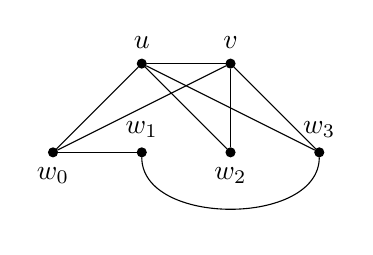
\begin{tikzpicture}
            \node[vertex, label=above:{$u$}] (u) at (0,0) {};
            \node[vertex, label=above:{$v$}, right=of u] (v) {};
            \node[vertex, label=above:{$w_1$}, below=of u] (w1) {};
            \node[vertex, label=below:{$w_2$}, right=of w1] (w2) {};
            \node[vertex, label=above:{$w_3$}, right=of w2] (w3) {};
            \node[vertex, label=below:{$w_0$}, left=of w1] (w0) {};

            \draw (u) -- (v);
            \draw (u) -- (w0);
            \draw (v) -- (w0);
            \draw (u) -- (w2);
            \draw (v) -- (w2);
            \draw (u) -- (w3);
            \draw (v) -- (w3);

            \draw (w0) -- (w1);
            \draw (w1) to[out=270, in=270] (w3);
        \end{tikzpicture}
    \end{figure}
\end{frame}

\begin{frame}{Reducing thinness instances}
    \begin{block}{Lemma 2}
        If three \textbf{non-adjacent} vertices have the same neighborhood, removing one of them does not modify the thinness of the graph.
    \end{block}

    \begin{figure}
        \centering
        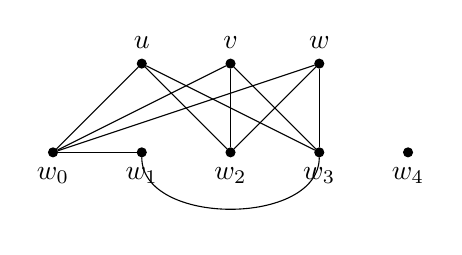
\begin{tikzpicture}
            \node[vertex, label=above:{$u$}] (u) at (0,0) {};
            \node[vertex, label=above:{$v$}, right=of u] (v) {};
            \node[vertex, label=above:{$w$}, right=of v] (w) {};
            \node[vertex, label=below:{$w_1$}, below=of u] (w1) {};
            \node[vertex, label=below:{$w_2$}, right=of w1] (w2) {};
            \node[vertex, label=below:{$w_3$}, right=of w2] (w3) {};
            \node[vertex, label=below:{$w_4$}, right=of w3] (w4) {};
            \node[vertex, label=below:{$w_0$}, left=of w1] (w0) {};

            \draw (u) -- (w0);
            \draw (v) -- (w0);
            \draw (w) -- (w0);
            \draw (u) -- (w2);
            \draw (v) -- (w2);
            \draw (w) -- (w2);
            \draw (u) -- (w3);
            \draw (v) -- (w3);
            \draw (w) -- (w3);

            \draw (w0) -- (w1);
            \draw (w1) to[out=270, in=270] (w3);
        \end{tikzpicture}
    \end{figure}
\end{frame}

\begin{frame}{Reducing thinness instances}
    What if the graph had few vertices after applying Lemmas 1 and 2 exhaustively? 

    \vspace{1em}
    \pause
    Say, at most $g(k)$ vertices for some $k$?

    \vspace{1em}
    \pause
    \textbf{What would that $k$ measure?}
\end{frame}

\section{Cluster module number}
\subsection{Modules}
\begin{frame}{Modules}
    \begin{block}{Definition (Module)}
        A \emph{module} of a graph $G$ is a subset $W$ of $V(G)$ such that every vertex outside $W$ is either adjacent to all vertices in $W$ or to none of them.
    \end{block}

    \begin{center}
        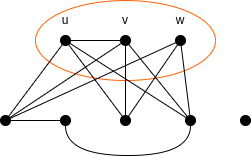
\includegraphics[width=0.5\textwidth]{img/module.png}
    \end{center}
\end{frame}

\subsection{Cluster modules}
\begin{frame}{Cluster modules}
    \begin{block}{Definition (Clique)}
        A \emph{clique} is a subset $C$ of vertices such that every vertex in $W$ is adjacent to all other vertices in $W$.
    \end{block}

    \begin{figure}
        \centering

        \tikz \graph[nodes={vertex}, empty nodes, edges={-}] { 
            subgraph K_n [n=5, clockwise]
        };
    \end{figure}
\end{frame}


\begin{frame}{Cluster modules}
    \begin{block}{Definition (Cluster)}
        A \emph{cluster} is a subset $C$ of vertices that induces a union of cliques.
    \end{block}
        
    \begin{center}
        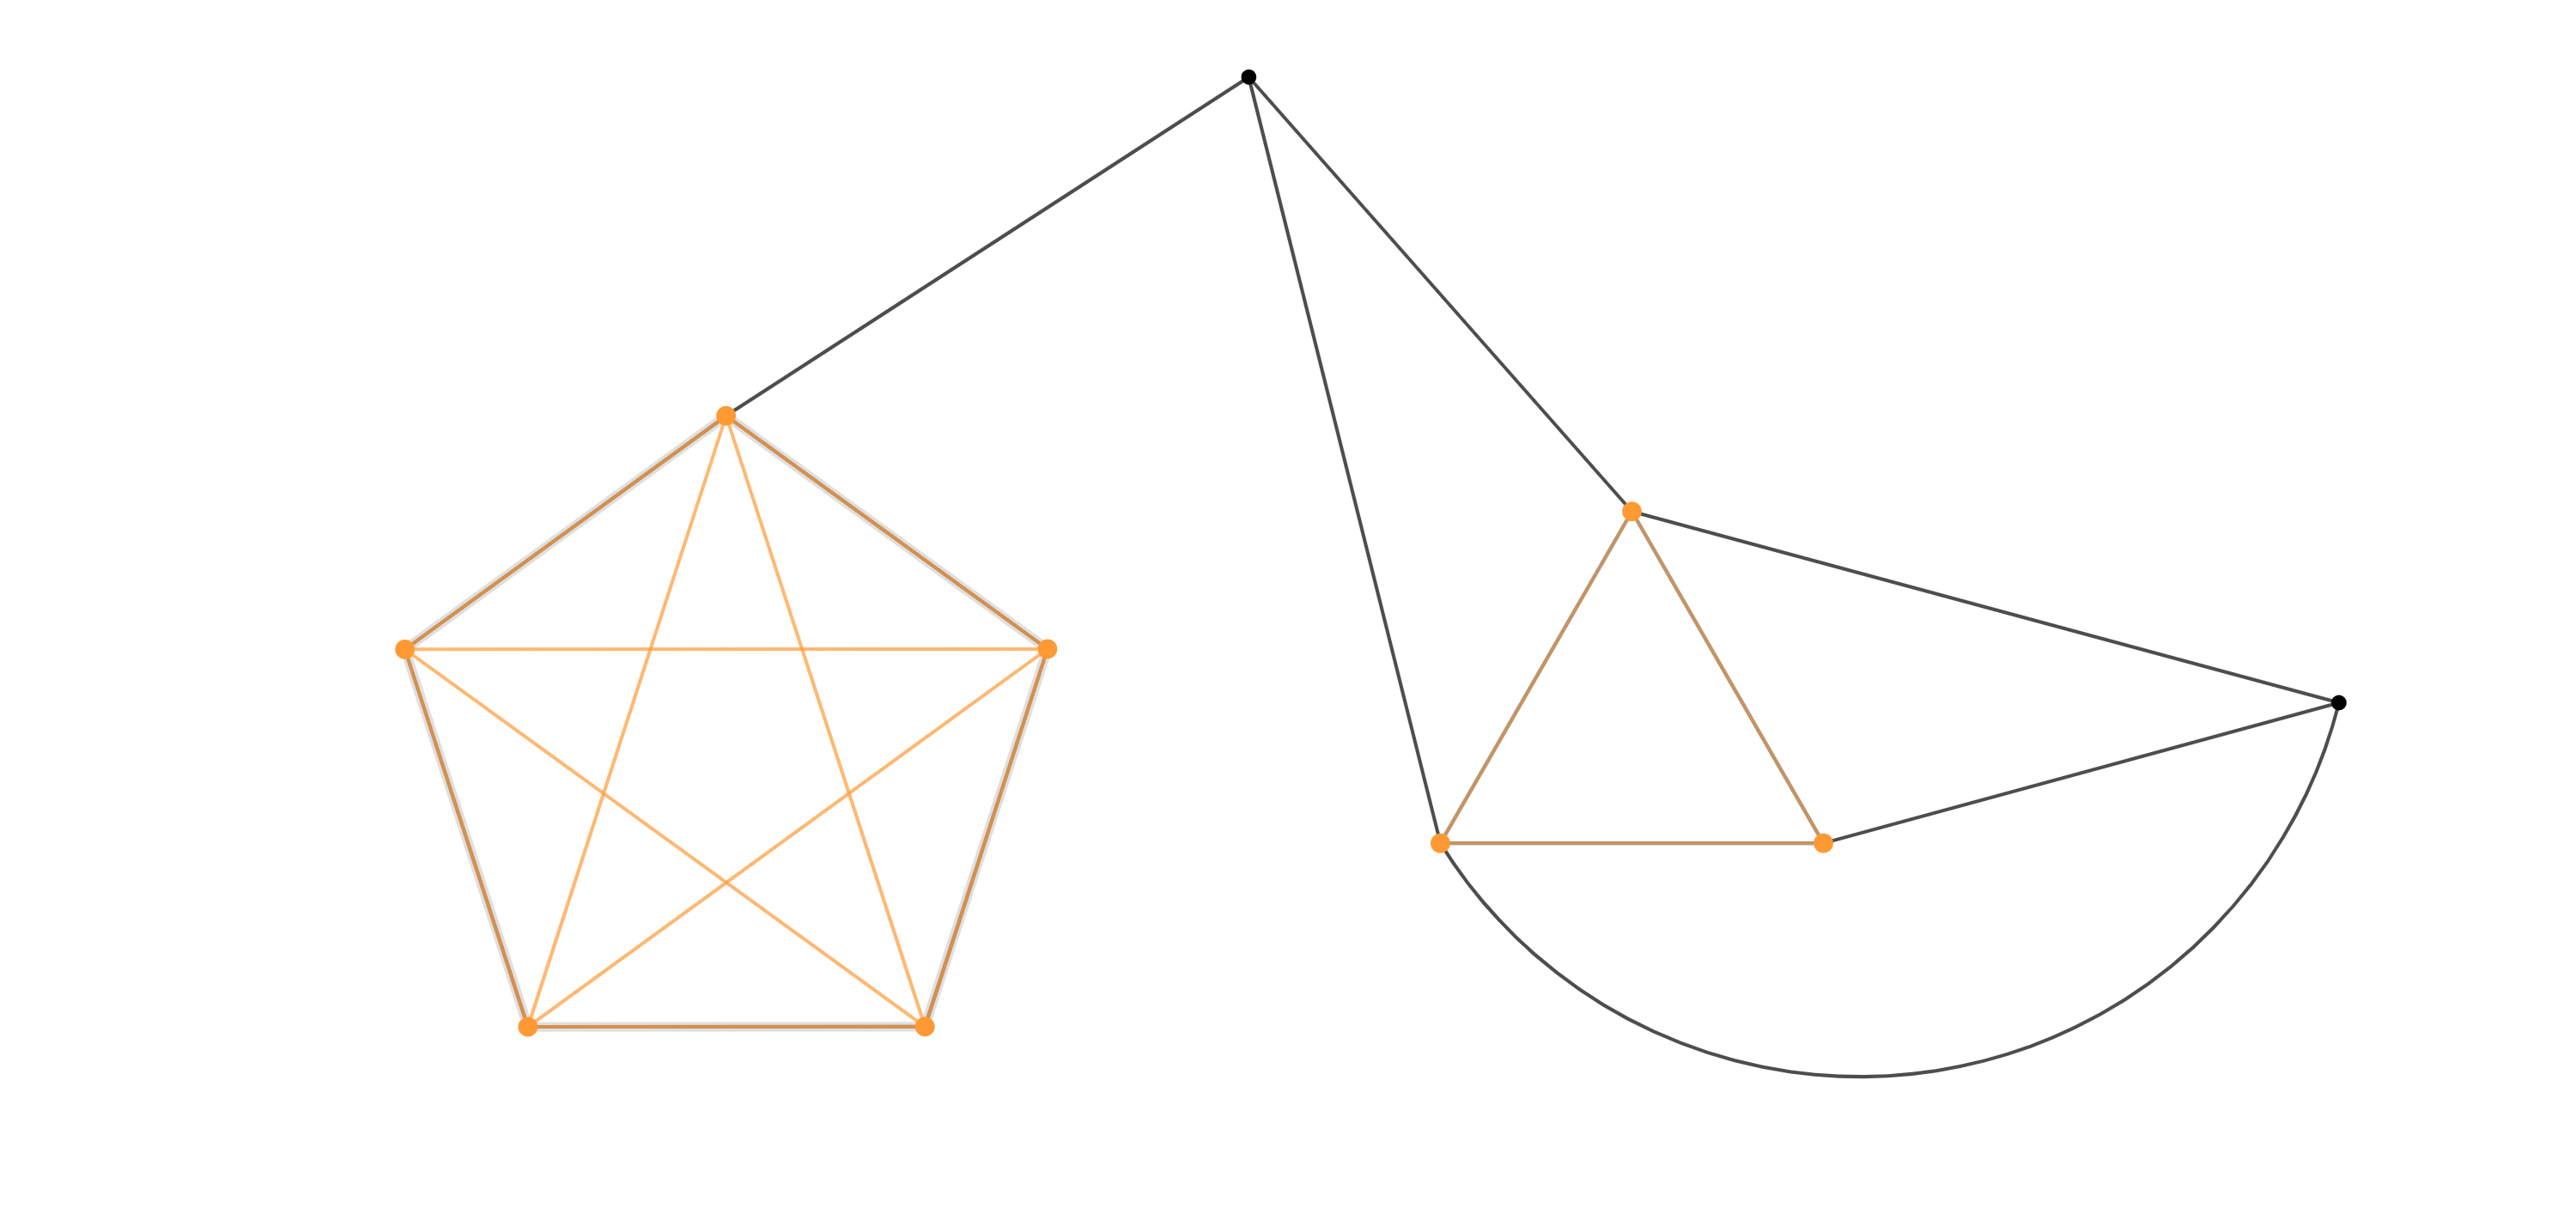
\includegraphics[width=1\textwidth]{img/cluster.png}
    \end{center}
\end{frame}

\begin{frame}{Cluster modules}
    \begin{block}{Definition (Cluster module)}
        A \emph{cluster module} is a subset $C$ of vertices that is a cluster and a module of $G$.
    \end{block}

    \begin{center}
        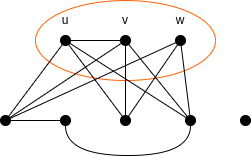
\includegraphics[width=0.5\textwidth]{img/module.png}
    \end{center}
\end{frame}

\subsection{Cluster module number}
\begin{frame}{Cluster module number}
    \begin{columns}
        \begin{column}{0.5\textwidth}
            \begin{block}{Definition}
                A \emph{cluster module partition} of a graph $G$ is a partition of the vertices of $G$ into cluster modules.
            \end{block}

            \begin{block}{Definition}
                The \emph{cluster module number} $\cm(G)$ of a graph $G$ is the minimum size of a cluster module partition of $G$.
            \end{block}
        \end{column}

        \begin{column}{0.5\textwidth}
            \begin{center}
                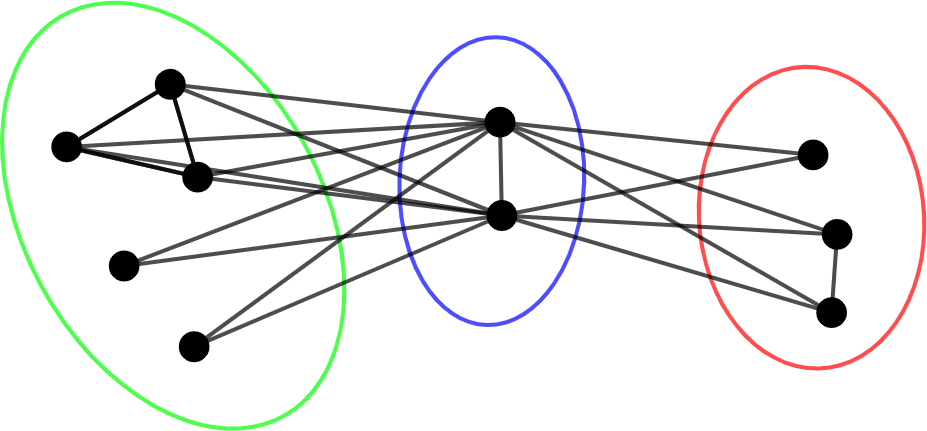
\includegraphics[width=\textwidth]{img/cluster_module_partition.png}
            \end{center}
        \end{column}
    \end{columns}
\end{frame}

\begin{frame}{Cluster module number}
    \begin{block}{Theorem}
        The cluster module number of a graph can be calculated in linear time.
    \end{block}
\end{frame}

\section{Parameterizations}
\subsection{Cluster module number}
\begin{frame}{Cluster module number}
    \begin{block}{Theorem}
        \textsc{Thinness} admits a kernel of size $2 \cdot \cm(G)$ when parameterized by the cluster module number of $G$.
    \end{block}
\end{frame}

\begin{frame}{Cluster module number}
    \framesubtitle{Proof}
    \begin{enumerate}
        \item Obtain an optimal cluster module partition of $G$.
    \end{enumerate}

    \begin{center}
    $\vimage[width=0.35\textwidth]{img/graph_with_cluster_module_partition.png}\ \varrow\ \vimage[width=0.4\textwidth]{img/cluster_module_partition.png}$
    \end{center}

\end{frame}

\begin{frame}{Cluster module number}
    \framesubtitle{Proof}
    \begin{enumerate}
        \item Obtain an optimal cluster module partition of $G$.
        \item (Lemma 1) Remove all vertices but one of each clique in each part of the cluster module partition.
    \end{enumerate}

    \begin{center}
        $\vimage[width=0.4\textwidth]{img/cluster_module_partition.png}\ \varrow\ \vimage[width=0.4\textwidth]{img/cluster_module_partition_lemma_1.png}$
    \end{center}
\end{frame}

\begin{frame}{Cluster module number}
    \framesubtitle{Proof}
    \begin{enumerate}
        \item Obtain an optimal cluster module partition of $G$.
        \item (Lemma 1) Remove all vertices but one of each clique in each part of the cluster module partition.
        \item (Lemma 2) Remove all vertices until only two of each part remain.
    \end{enumerate}
    
    \begin{center}
        $\vimage[width=0.4\textwidth]{img/cluster_module_partition_lemma_1.png}\ \varrow\ \vimage[width=0.4\textwidth]{img/cluster_module_partition_lemma_2.png}$
    \end{center}
\end{frame}


\begin{frame}{Cluster module number}
    \framesubtitle{Proof}
    The resulting graph is $k$-thin if and only if the original graph is $k$-thin, and it has at most $2 \cdot \cm(G)$ vertices. Thus, this is a \textbf{kernel} of size $2 \cdot \cm(G)$.
    \begin{center}
        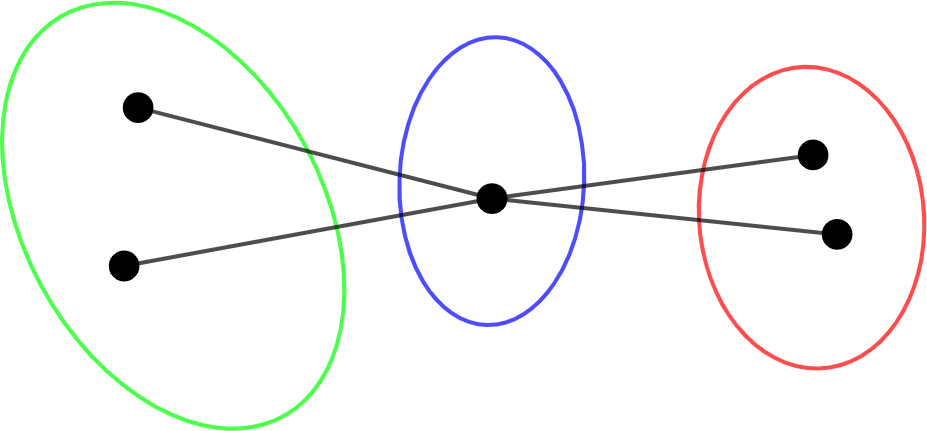
\includegraphics[width=0.4\textwidth]{img/cluster_module_partition_lemma_2.png}
    \end{center}
\end{frame}


\subsection{Neighborhood diversity}
\begin{frame}{Neighborhood type}
    \begin{block}{Definition (Neighborhood type)}
        Two vertices $v$ and $w$ have the same \emph{neighborhood type} if $N(v) \setminus \{w\} = N(w) \setminus \{v\}$.
    \end{block}

    \begin{figure}
        \centering
        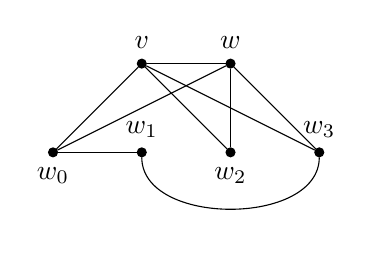
\begin{tikzpicture}
            \node[vertex, label=above:{$v$}] (u) at (0,0) {};
            \node[vertex, label=above:{$w$}, right=of u] (v) {};
            \node[vertex, label=above:{$w_1$}, below=of u] (w1) {};
            \node[vertex, label=below:{$w_2$}, right=of w1] (w2) {};
            \node[vertex, label=above:{$w_3$}, right=of w2] (w3) {};
            \node[vertex, label=below:{$w_0$}, left=of w1] (w0) {};

            \draw (u) -- (v);
            \draw (u) -- (w0);
            \draw (v) -- (w0);
            \draw (u) -- (w2);
            \draw (v) -- (w2);
            \draw (u) -- (w3);
            \draw (v) -- (w3);

            \draw (w0) -- (w1);
            \draw (w1) to[out=270, in=270] (w3);
        \end{tikzpicture}
    \end{figure}
\end{frame}

\begin{frame}{Neighborhood partition}
    \begin{block}{Definition (Neighborhood partition, Neighborhood diversity)}
        A partition of the vertices of a graph $G$ is a \emph{neighborhood partition} if every two vertices in the same part have the same neighborhood type. The \emph{neighborhood diversity} $\nd(G)$ of $G$ is the minimum number of parts in a neighborhood partition of $G$.
    \end{block}
    \begin{center}
        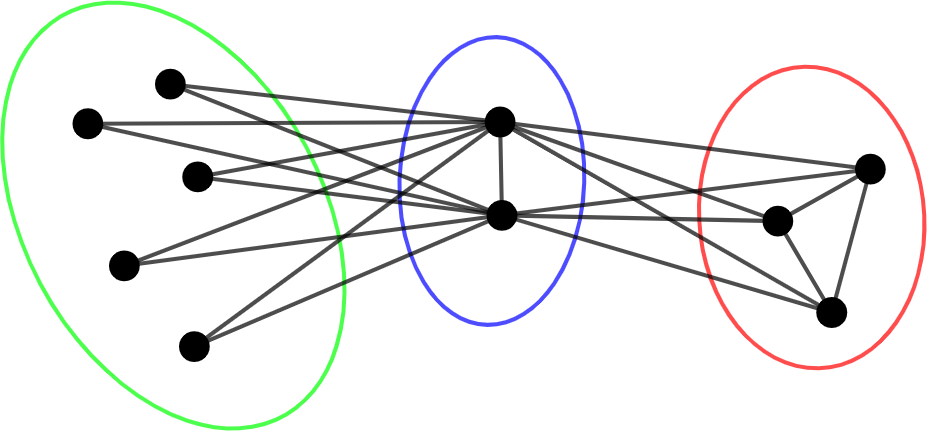
\includegraphics[width=0.4\textwidth]{img/neighborhood_partition.png}
    \end{center}
\end{frame}

\begin{frame}{Neighborhood diversity}
    \begin{block}{Lemma (\cite{neighborhood-diversity})}
        Every part of a neighborhood partition is either a clique or an independent set.
    \end{block}

    \begin{center}
        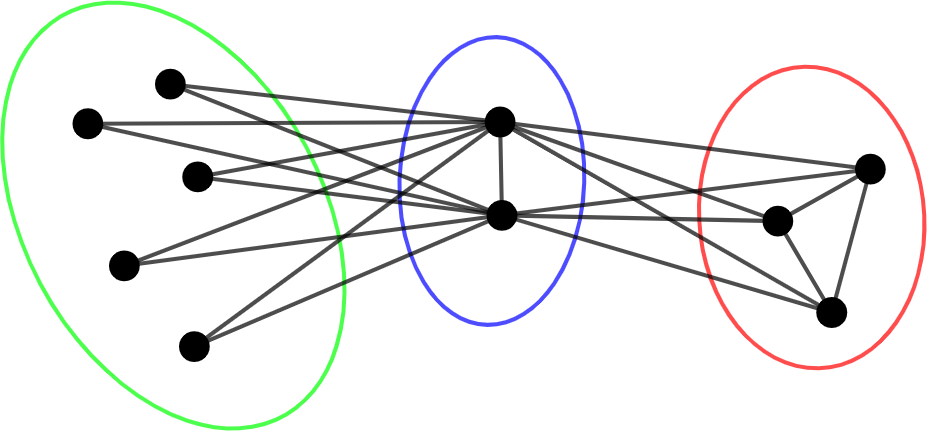
\includegraphics[width=0.4\textwidth]{img/neighborhood_partition.png}
    \end{center}
\end{frame}

\begin{frame}{Neighborhood diversity}
    \begin{block}{Lemma}
        $\cm(G) \leq \nd(G)$.
    \end{block}
    \pause
    \vspace{1em}
    We can then use the same kernelization algorithm as for the cluster module number to obtain a kernel of size at most $2 \cdot \nd(G)$ for \textsc{Thinness} parameterized by the neighborhood diversity of $G$.
\end{frame}

\subsection{Twin-cover}
\begin{frame}{Twin-cover}
    \begin{columns}
        \begin{column}{0.5\textwidth}
            \begin{block}{Definition (Twin-cover)}
                A subset $X$ of vertices of $G$ is a \emph{twin-cover} if for every edge $(u, v)$ of $E(G)$, either
                \begin{itemize}
                    \item one of $\{u, v\}$ belongs to $X$, or
                    \item $u$ and $v$ are twins, meaning, $N[u] = N[v]$.
                \end{itemize}

                The \emph{twin-cover number} $\tc(G)$ of $G$ is the minimum size of a twin-cover of $G$.
            \end{block}
        \end{column}
        \begin{column}{0.5\textwidth}
            \begin{center}
                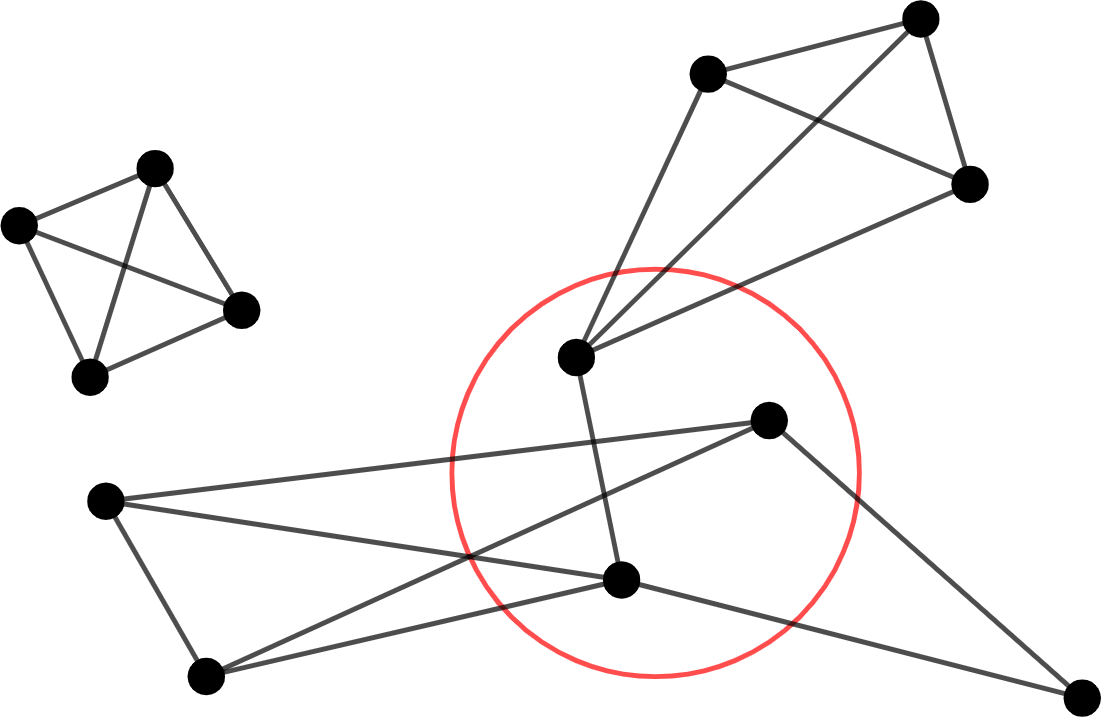
\includegraphics[width=\textwidth]{img/twin-cover.png}
            \end{center}
        \end{column}
    \end{columns}
\end{frame}

\begin{frame}{Twin-cover}
    \begin{block}{Lemma}
        $\cm(G) \leq 2^{\tc(G)} + \tc(G)$.
    \end{block}

    \textcolor{blue}{Proof:} We create $\tc(G)$ parts, one for each vertex in a twin-cover, and then partition the remaining vertices by their \textbf{neighborhoods in $\mathbf{X}$}.
    
    \begin{center}
        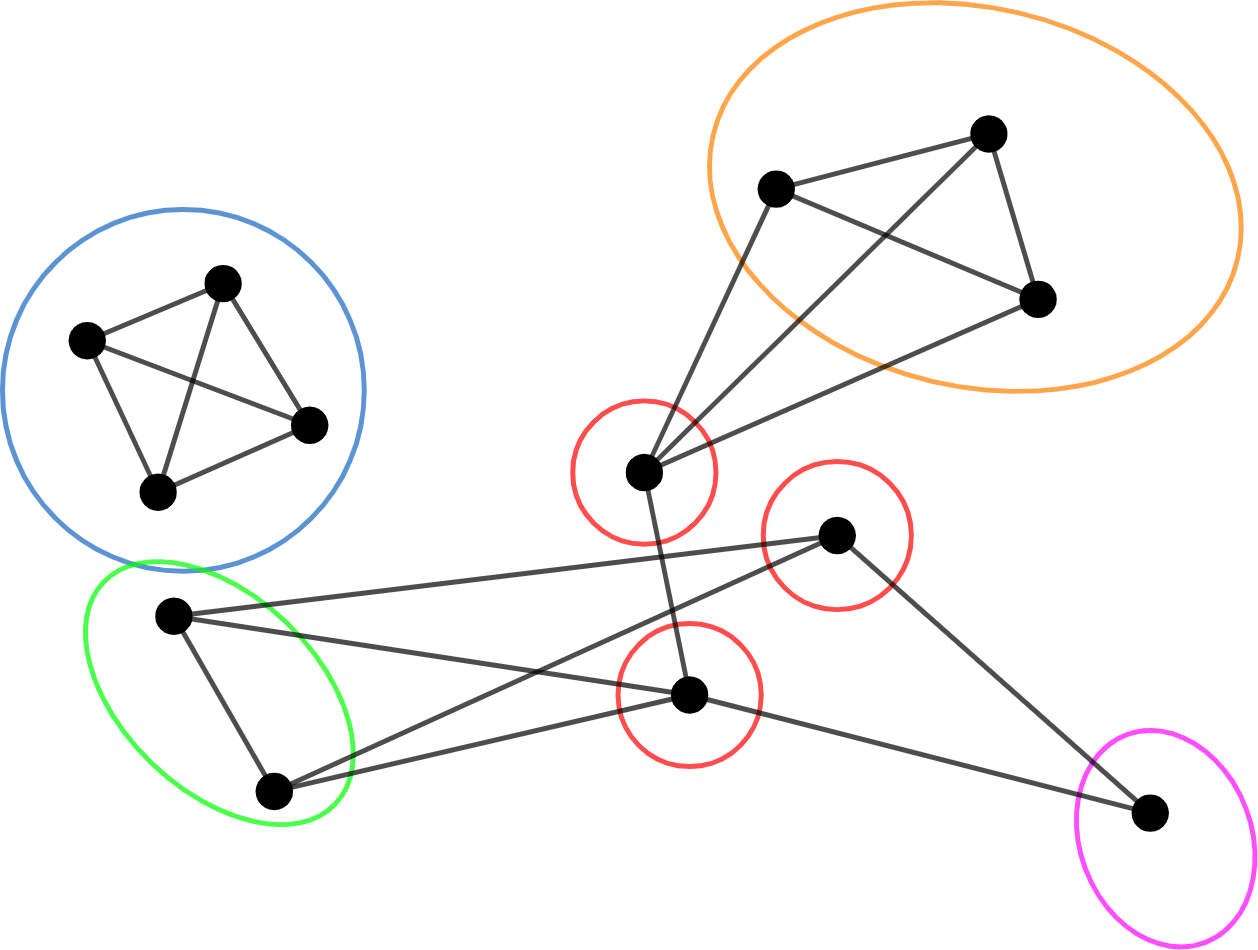
\includegraphics[width=0.45\textwidth]{img/twin-cover_cluster_module_partition.png}
    \end{center}
\end{frame}


\begin{frame}{Twin-cover}
    We can again use the same kernelization algorithm to obtain a kernel of size at most $2 \cdot (2^{\tc(G)} + \tc(G))$ for \textsc{Thinness} parameterized by the twin-cover number of $G$.
\end{frame}

\subsection{Vertex cover}
\begin{frame}{Vertex cover}
    \begin{block}{Definition}
        A \emph{vertex cover} of a graph $G$ is a subset $S$ of vertices such that every edge of $G$ is incident to at least one vertex in $S$.

        The \emph{vertex cover number} $\vc(G)$ of $G$ is the minimum size of a vertex cover of $G$.
    \end{block}
    
    \begin{center}
        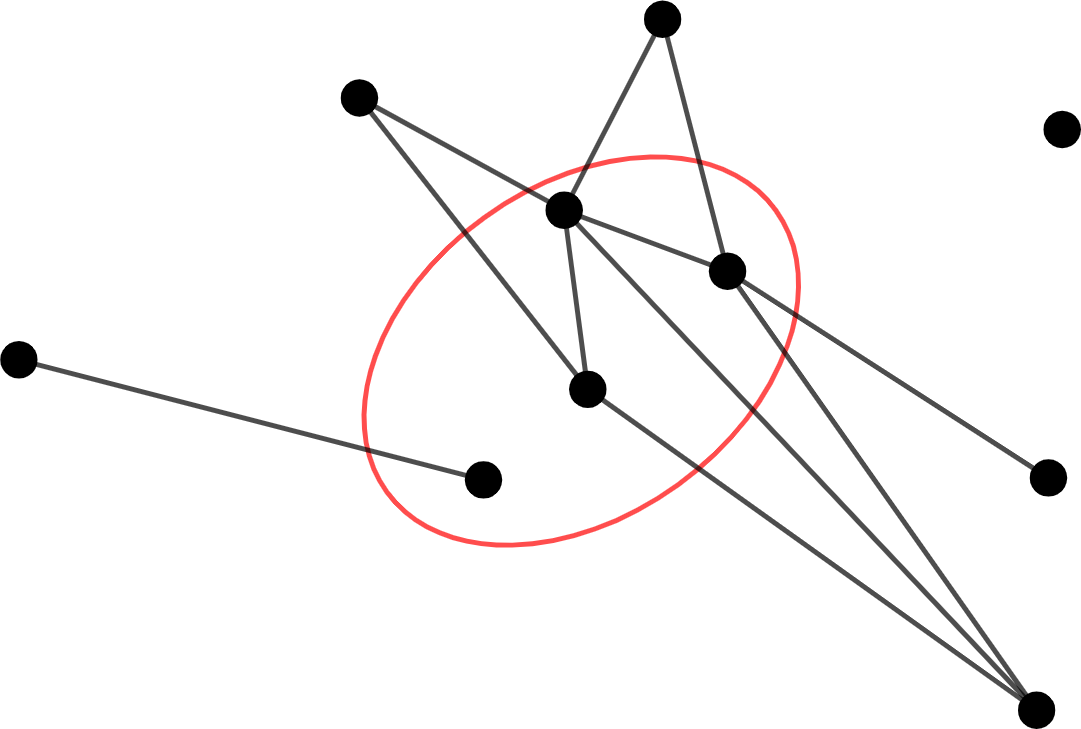
\includegraphics[width=0.45\textwidth]{img/vertex_cover.png}
    \end{center}
\end{frame}

\begin{frame}{Vertex cover}
    Every vertex cover is a twin-cover.
    We can use the same kernelization algorithm to obtain a kernel of size at most $2 \cdot (2^{\vc(G)} + \vc(G))$ for \textsc{Thinness} parameterized by the vertex cover number of $G$.
\end{frame}

\subsection{Kernelization lower bounds}
\begin{frame}{Kernel size}
    The kernels when parameterized by cluster module number and neighborhood diversity have \textbf{linear size} in the parameter, while the kernels when parameterized by twin-cover and vertex cover number have \textbf{exponential size} in the parameter.


\end{frame}

\begin{frame}{Size lower bound}
    \begin{block}{Theorem}
        Let $\p$ be a graph parameter such that
        \begin{itemize}
            \item for every graph $G$, we have $\p(G) \leq \abs{V(G)}$, and
            \item if $H$ is the disjoint union of two graphs $G_1$ and $G_2$, we have $\p(H) \leq \max\{\p(G_1), \p(G_2)\}$.
        \end{itemize}
        Then \textsc{Thinness} parameterized by $\p$ has no polynomial kernel assuming $\textsf{NP} \not\subseteq \textsf{coNP} / \textsf{poly}$.
    \end{block}
\end{frame}

\begin{frame}{Size lower bound}
    This does not apply when parameterizing \textsc{Thinness} by the twin-cover or the vertex cover, but it does apply when parameterizing by
    \begin{itemize}
        \item treewidth,
        \item bandwidth,
        \item \textbf{thinness,}
        \item \dots and many more.
    \end{itemize}
\end{frame}

\section*{References}
\begin{frame}{References}
    \tiny
    \bibliographystyle{plain}
    \bibliography{references}
\end{frame}

{
    \definecolor{ceruleanblue}{rgb}{0.23, 0.28, 0.75}
    \setbeamertemplate{background canvas}{%
    \begin{tikzpicture}[remember picture,overlay]
    \shade[top color=ceruleanblue,bottom color=black,middle color=ceruleanblue]
    (current page.north west)
        rectangle
    (current page.south east);
    \end{tikzpicture}%     
    }
    \setbeamercolor{background canvas}{bg=ceruleanblue}
    \begin{frame}[plain]
        \centering
        \usebeamerfont{title}
        {\Huge
        \textcolor{white}{Thank you!}
        }
        
    \end{frame}
}

\end{document}
